\documentclass{beamer}
\usetheme{Warsaw}
\useinnertheme{circles}
\useoutertheme[subsection=false]{smoothbars}
\usepackage[utf8x]{inputenc}
\usepackage[czech]{babel}
\usepackage[T1]{fontenc}
\usepackage{listings}

\begin{document}

\AtBeginSection[]
{
  \begin{frame}
    \frametitle{Outline}
    \tableofcontents[currentsection]
  \end{frame}
}

\title{Open source programování}
\subtitle{Úvod do open source}
\author{Petr Baudiš $\langle${\tt pasky@ucw.cz}$\rangle$}
\institute{MFF UK 2011\\
	\vskip 1ex
	\pgfdeclareimage[height=4ex]{ccbysa}{by-sa.pdf}
	\pgfuseimage{ccbysa}
}
\date{}
\frame{\titlepage}

\section{Úvod}

\subsection{}
\begin{frame}{Úžasný nový svět\dots}
\begin{center}
{\bf Open source}
\end{center}
\begin{itemize}
\item Otevřený zdrojový kód
\item Právo na jeho úpravy a redistribuci upravené verze
\item (Povinnost umožnit ostatním úpravy i té své verze)
\end{itemize}
\begin{center}

\includegraphics[width=2cm]{opensource-rgb.pdf}\hskip 1em

\includegraphics[width=2cm]{heckert_gnu.pdf}\hskip 1em

\includegraphics[width=2cm]{cc.pdf}
\end{center}
\end{frame}

\subsection{}
\begin{frame}{Proč a o čem}
\begin{itemize}
\item Můžete zlepšit svět!
\item Můžete zlepšit sebe!
\item Nebo alespoň zjistit, proč to nefunguje.
\pause
\vskip 4ex
\item Filosofie open source, licence
\item Jak využít otevřených zdrojových kódů
\item Jak přežít v open source komunitě
\pause
\vskip 4ex
\item Betaverze. :-) Fork me on Github! {\tt https://github.com/pasky/oss-lec}
\end{itemize}
\end{frame}

\subsection{}
\begin{frame}{Váš úkol}
\begin{itemize}
\item {\bf Cíl hry:} Prosadit nějakou svoji změnu do nějakého upstreamu
\item Vyberte si projekt a něco užitečného a netriviálního\\do něj naimplementujete.
\item Je nutná průběžná práce během semestru!
\vskip 4ex
\item Zápočet: Dvě prezentace během semestru\\(co budete dělat; jak to dopadlo)
\item Zkouška: Rozhovor nad osudy vašeho patche
\end{itemize}
\end{frame}

\subsection{}
\begin{frame}{Průběh semestru}
\begin{itemize}
\item {\em Úvod do praktického hackování}
\item Úvod do open source systémů
\item Přehlídka open source projektů
\item {\bf Prezentace č. 1}
\item Vývoj software v open source prostředí
\item {\em Úvod do správy verzí a nástroje git}
\item Autorské právo
\item Správa open source projektů, komerce a open source,\\open hardware
\item {\bf Prezentace č. 2}
\end{itemize}
\end{frame}

\subsection{}
\begin{frame}{Reference}
\begin{itemize}
\item {\tt http://pasky.or.cz/vyuka/2011-PRG055}
\item The Cathedral and the Bazaar, atd.
\vskip 4ex
\item {\em Programování v UNIXu}, {\em Linux kernel}
\item {\em Open source programování} na FEL ČVUT
\item Summer of Code
\end{itemize}
\end{frame}

\subsection{}
\begin{frame}{O čem dnes}
\begin{itemize}
\item Historie open source a důležité záchytné body
\item Infrastruktura pro open source projekty
\item Kuchařka na výrobu a přijetí patche
\end{itemize}
\end{frame}


\section{Open source}

\subsection{}
\begin{frame}{Historie}
\begin{columns}
\begin{column}{2cm}
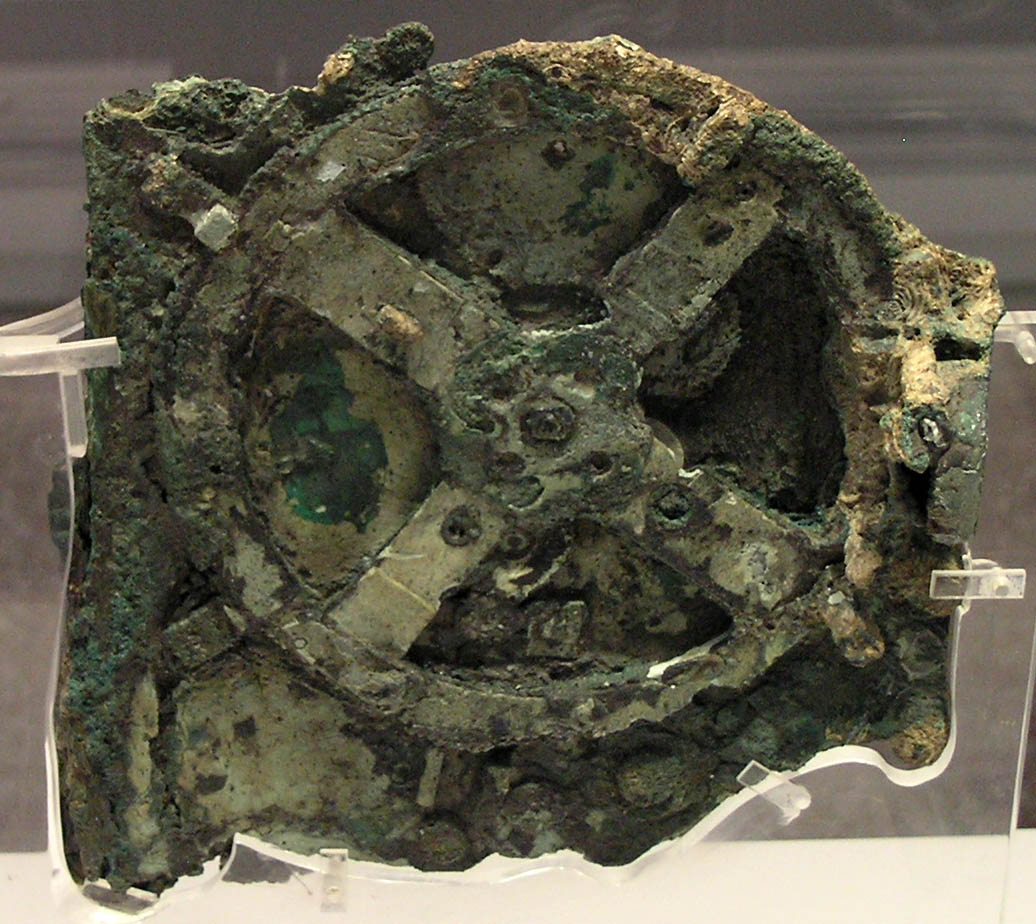
\includegraphics[width=2cm]{antikythera.jpg}
\vskip 3ex
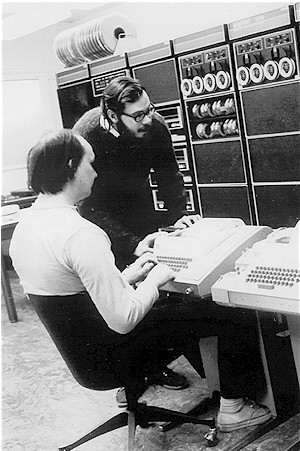
\includegraphics[width=2cm]{pdp11.jpg}
\end{column}
\begin{column}{9cm}
\begin{itemize}
\item Antikythera (150--100 př.n.l.) --- antické hi-tech hodiny, astronomicky přesný pohyb měsíce, dokumentace na plášti přístroje
\item UNIX (70. léta 20. stol.) --- distribuován na páskách, samozřejmě včetně zdrojových kódů
\item Closed source software --- na vzestupu, jak software přestává být příslušenstvím počítače a stává se portabilním
\item 386BSD opět otevřelo (přepsaný) UNIXový kód,\\ovšem mezitím vzniká i GNU a Linux
\end{itemize}
\end{column}
\end{columns}
\end{frame}

\subsection{}
\begin{frame}{Internet}
\begin{itemize}
\item Komunikace (USENET, e-mail, IRC) umožnila celosvětovou spolupráci programátorů (podobný efekt jako o 30 let později Wikipedie)
\item Vzniká {\em hackerská kultura}, kde je přístup ke zdrojovým kódům důležitý atribut
\end{itemize}
\pause
\vskip 2ex
\begin{columns}
\begin{column}{8cm}
\begin{itemize}
\item Internet (vznikající z ARPAnetu)\\je zcela otevřený systém
\item Specifikace protokolů veřejně publikovány jako {\em Requests for Comment},\\otevřený proces standardizace
\item Jon Postel: ``Be conservative in what you send, liberal in what you accept.''
\end{itemize}
\end{column}
\begin{column}{4cm}
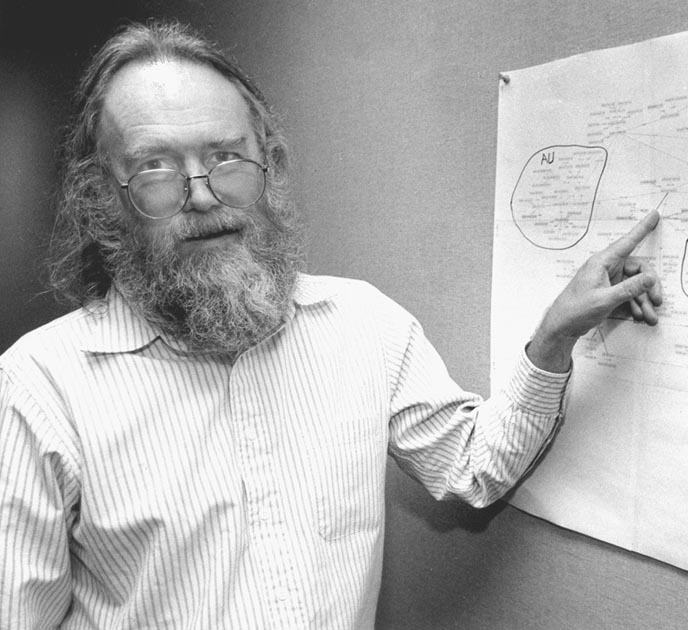
\includegraphics[width=4cm]{Jon_Postel.jpg}
\end{column}
\end{columns}
\end{frame}

\subsection{}
\begin{frame}{GNU a Free Software Foundation}
\begin{columns}
\begin{column}{9cm}
\begin{itemize}
\item Richard M. Stallman (MIT AI labs):
Už ani software pro tiskárnu si člověk nemůže přiohnout?
\item 1983 zakládá GNU, 1985 vzniká FSF
\item {\em Svobodný software} může kdokoliv modifikovat, pokud tuto možnost zachová i pro ostatní (``copyleft'').
Neomezené použití i prodej.
\item {\em General Public Licence} (GPL), {\em Lesser GPL}, {\em GFDL}.
\item GNU: Základní nástroje, textový editor, překladač, nyní i editor obrázků atd.
\item Jádro dodal Linus Torvalds $\Rightarrow$ GNU/Linux (ale\dots)
\vskip 2ex
\item<2> Nesvobodný software může být dokonce amorální --- {\bf politicko-společenská agenda.}
\end{itemize}
\end{column}
\begin{column}{2cm}
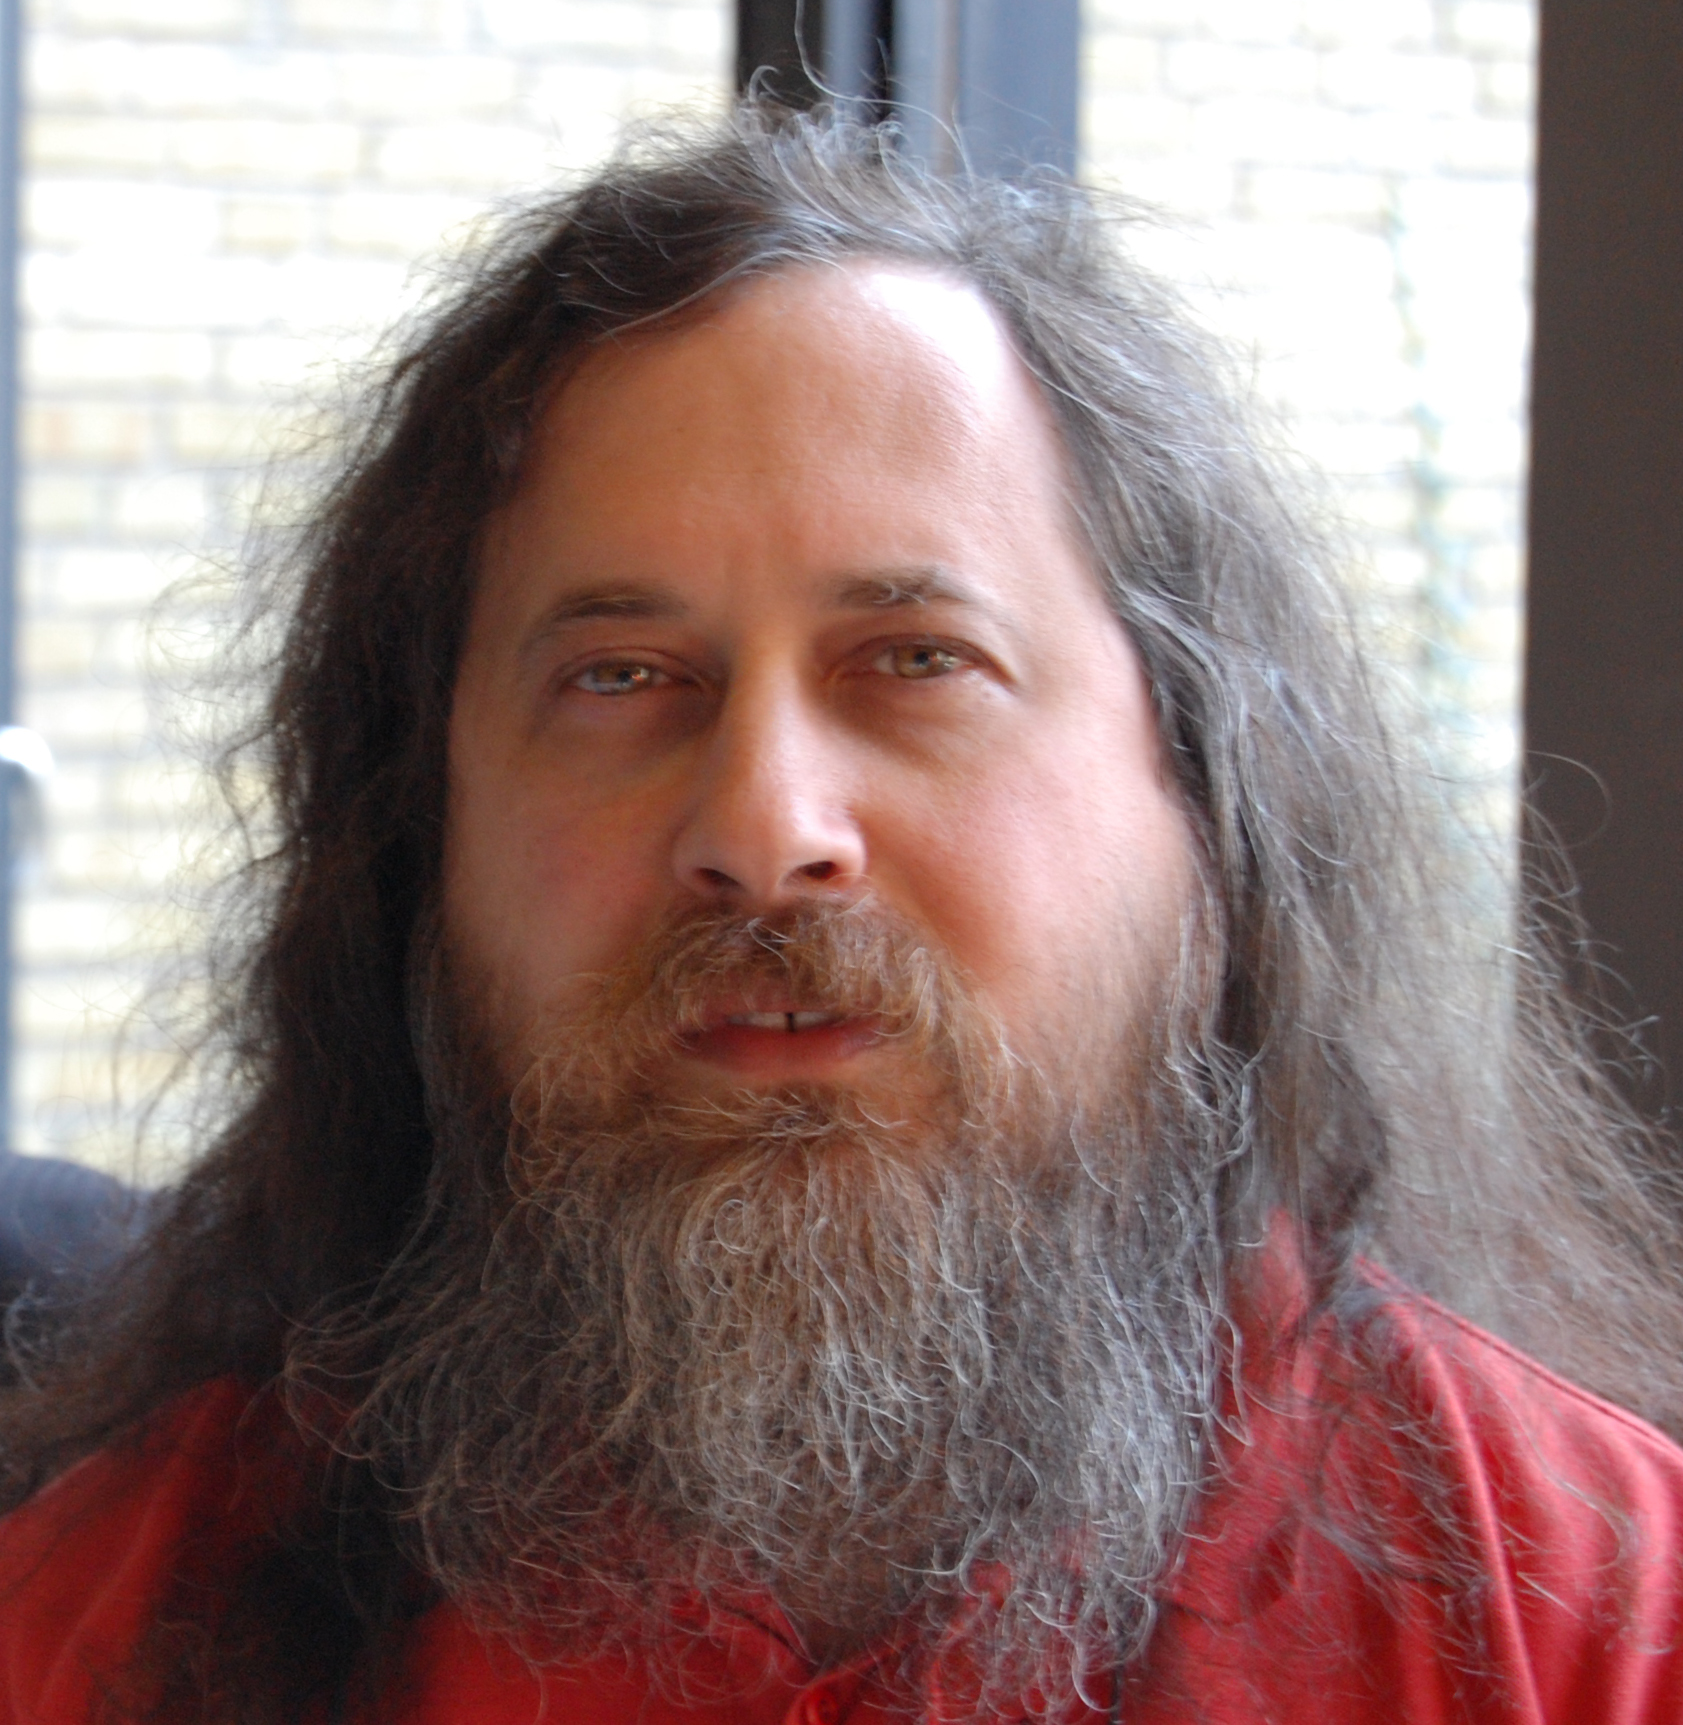
\includegraphics[width=2cm]{rms.jpg}
\vskip 8ex

\includegraphics[width=2cm]{heckert_gnu.pdf}
\end{column}
\end{columns}
\end{frame}

\subsection{}
\begin{frame}{Open Source Initiative}
\begin{columns}
\begin{column}{4cm}

\includegraphics[width=4cm]{opensource-rgb.pdf}
\end{column}
\begin{column}{7cm}
\begin{itemize}
\item Svobodný software omezuje individuální svobodu ``ve prospěch společnosti'' --- upravená verze musí být pod stejnou licencí
\item Alternativa --- BSD / MIT / X11 apod. licence; krátká, stručná,\\dělejte si se zdrojáky co chcete
\item Open source zahrnuje kromě svobodného software i tyto licence
\item Open Source Initiative (Bruce Perens, Eric S. Raymond) --- odklon od moralizování, buďme pragmatičtí!
\end{itemize}
\end{column}
\end{columns}
\end{frame}

\subsection{}
\begin{frame}{Creative Commons}
\begin{columns}
\begin{column}{4cm}

\includegraphics[width=4cm]{cc.pdf}
\end{column}
\begin{column}{7cm}
\begin{itemize}
\item Softwarové licence se na jiný obsah moc nehodí
\item Několik srozumitelných variant pro tvůrce obsahu:
\begin{itemize}
\item BY (attribution)
\item NC (non-commercial)
\item SA (share alike; zase copyleft!)
\item ND (no derivative works)
\end{itemize}
\item {\em Svobodná kultura} --- nespočet fotografií, hudby, další tvorby;\\``poster child'' je {\bf Wikipedie}
\end{itemize}
\end{column}
\end{columns}
\end{frame}

\subsection{}
\begin{frame}{Současnost}
\begin{columns}
\begin{column}{7cm}
\begin{itemize}
\item Internet z velké části stojí na OSS --- infrastruktura i služby
\item Linux v řadě embedded zařízení (routery, MP3 přehrávače, Android)
\item I velké podniky, akademický sektor, občas domácí počítače
\vskip 2ex
\item Open source software běžný i na Windows (Firefox, VLC, LibreOffice)
\item Nejen software: Projekt Guttenberg, Wikipedie, Thingiverse
\vskip 2ex
\item Softwarové patenty, kontroverzní trademarky, web a (A)GPLv3.
\end{itemize}
\end{column}
\begin{column}{4cm}
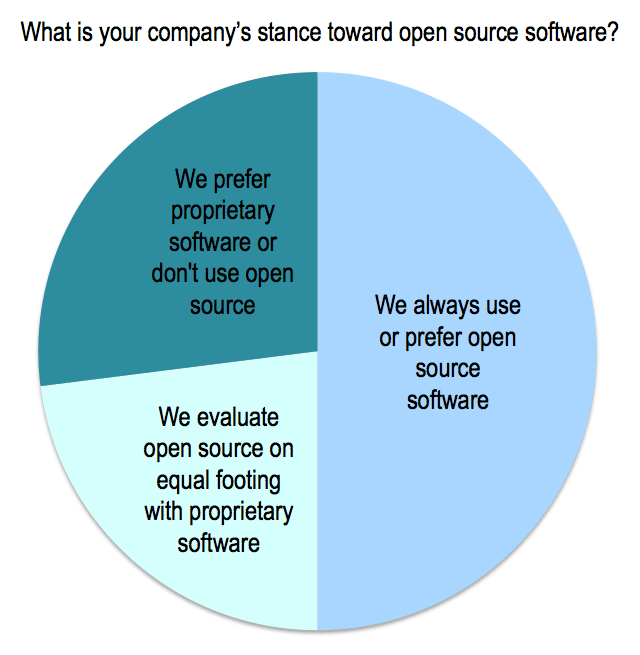
\includegraphics[width=4cm]{Prefer-Or-Prevent.png}
\end{column}
\end{columns}
\end{frame}


\section{Jak se vyvíjejí projekty}

\subsection{}
\begin{frame}{Základní infrastruktura}
\begin{itemize}
\item {\em Místo, kde jsou zdrojáky}
\item Homepage projektu --- popis, novinky, download, dokumentace, vývoj
\item Komunikační zázemí --- mailing list nebo webové fórum,\\wiki, IRC
\item Vývojářské zázemí --- bugtracker, systém pro správu verzí
\item Index --- distribuce, FreshMeat (\dots, Code Search, Koders.com)
\end{itemize}
\end{frame}

\subsection{}
\begin{frame}{Kujme kód}
\begin{columns}
\begin{column}{7cm}
\begin{itemize}
\item Nutné zázemí, server + mnoho služeb \\ $\Rightarrow$ hostingy pro open source projekty
\item Sourceforge / Savannah, Google Code
\item Github / Gitorious, Bitbucket, Launchpad
\end{itemize}
\end{column}
\begin{column}{4cm}

\includegraphics[width=4cm]{meditate.png}
\end{column}
\end{columns}
\end{frame}


\section{Patchovací kuchařka}

\subsection{}
\begin{frame}{Chtěl bych si dopsat\dots}
\begin{itemize}
\item Sežeňte si zdrojáky. (Download z webu, {\tt apt-get source}, \dots)
\item Najděte to správné místo, pochopte konvence,\\držte se coding style. (Doxygen, {\tt HACKING}, \dots)
\item Zkompilujte projekt. (Nainstalujte závislosti,\\vývojářské verze knihoven, {\tt apt-get build-dep}, \dots;\\``svatá trojice'' {\tt ./configure; make; make install})
\item Zdokumentujte, co je třeba. Používá-li se unit testing,\\měli byste napsat testcase.
\end{itemize}
\end{frame}

\subsection{}
\begin{frame}{A chtěl bych, aby to mohli používat i ostatní}
\begin{itemize}
\item Vyrobte patch nebo sérii patchů.\\({\tt diff -u} nebo systém pro správu verzí)
\item Pošlete patch na mailing list.\\(Pozor na whitespace damage, zalamování.)
% TODO: logo githubu; licence?!
\item Github: Commit změn, fork, push, pull request.
\pause
\vskip 4ex
\item Nikdo během pár dní neodpověděl? Urgujte a vytrvejte.
\item Reagujte na připomínky a bugreporty. Buďte připraveni implementaci výrazně přepracovat.
\item Připomínkovat může ``kdokoliv'', poslední slovo má správce (nebo správci) projektu.
\item U některých projektů je nutný copyright assignment.
\end{itemize}
\end{frame}

\subsection{}
\begin{frame}{Potřebuji pomoc...}
\begin{itemize}
\item Nenapadá mne, na čem pracovat.
\item Nikdo si mne nevšímá a urgence nepomáhají.
\item Chtějí po mně nesmysly!
\item Nadává mi Ulrich Drepper.
\end{itemize}
\vskip 4ex
\begin{center}
{\tt pasky@ucw.cz}
\end{center}
\end{frame}

\end{document}
